% Shared style for all Git & GitHub lectures (same look as the N-body course)
\documentclass[11pt,a4paper]{article}
\usepackage[margin=2.3cm]{geometry}
\usepackage[T1]{fontenc}
\usepackage{lmodern}
\usepackage{upquote}   % straight quotes in monospaced text, so commands can be copied
\usepackage{microtype}
% keep '--' as two real hyphens in monospace text (commands like --version)
\DisableLigatures[-,<,>]{family=tt*}
\usepackage{booktabs,enumitem,graphicx,xcolor}
\usepackage{array}
\usepackage{needspace}
\usepackage{longtable}
\usepackage{float}
\usepackage{tikz}
\usetikzlibrary{arrows.meta,calc,positioning,decorations.pathreplacing,shapes.geometric,fit,backgrounds}
\usepackage[most]{tcolorbox}
\usepackage{listings}
\usepackage{fancyhdr}
\usepackage[colorlinks=true,linkcolor=blue!50!black,urlcolor=blue!50!black,citecolor=blue!50!black]{hyperref}

\setlength{\parindent}{0pt}
\setlength{\parskip}{0.6em}
\setlength{\abovecaptionskip}{4pt}
\usepackage[font=small,labelfont=bf]{caption}
\setlist{itemsep=0.2em,topsep=0.3em}

% ---------- colours ----------
\definecolor{cbg}{HTML}{F6F8FA}
\definecolor{ckw}{HTML}{0B5CAD}
\definecolor{ccm}{HTML}{6A737D}
\definecolor{cst}{HTML}{B5451B}
\definecolor{cpart}{HTML}{1F6FB2}
\definecolor{cheavy}{HTML}{C0392B}
\definecolor{cgreen}{HTML}{2E8B57}

% ---------- terminal listings ----------
% In a terminal session, lines starting with "$" are what YOU type.
% Everything else is what Git prints back.
\lstdefinestyle{term}{
  basicstyle=\ttfamily\small, backgroundcolor=\color{cbg},
  frame=single, rulecolor=\color{black!15}, showstringspaces=false,
  breaklines=true, columns=fullflexible, keepspaces=true,
  aboveskip=0.6em, belowskip=0.6em, xleftmargin=4pt, xrightmargin=4pt,
  literate={\$\ }{{\textcolor{cgreen}{\$\ }}}2,
  upquote=true
}
\lstset{style=term}
\newcommand{\code}[1]{\texttt{\small #1}}

% ---------- boxes ----------
\newtcolorbox{history}{colback=yellow!8,colframe=orange!60!black,
  title={History},fonttitle=\bfseries\small,left=4pt,right=4pt,top=2pt,bottom=2pt}
\newtcolorbox{quickfact}{colback=purple!4,colframe=purple!55!black,
  title={Quick fact},fonttitle=\bfseries\small,left=4pt,right=4pt,top=2pt,bottom=2pt}
\newtcolorbox{keyidea}{colback=blue!4,colframe=blue!50!black,
  title={Key idea},fonttitle=\bfseries\small,left=4pt,right=4pt,top=2pt,bottom=2pt}
\newtcolorbox{pitfall}{colback=red!4,colframe=red!55!black,
  title={Pitfall},fonttitle=\bfseries\small,left=4pt,right=4pt,top=2pt,bottom=2pt}
\newtcolorbox{tryit}{colback=teal!5,colframe=teal!55!black,
  title={Try it},fonttitle=\bfseries\small,left=4pt,right=4pt,top=2pt,bottom=2pt,breakable}
\newtcolorbox{homework}[1]{colback=green!4,colframe=green!40!black,
  title={Homework #1},fonttitle=\bfseries\small,left=4pt,right=4pt,top=2pt,bottom=2pt,
  breakable}
\newtcolorbox{goals}{colback=gray!6,colframe=gray!60!black,
  title={Learning goals},fonttitle=\bfseries\small,left=4pt,right=4pt,top=2pt,bottom=2pt}

% Solutions always start on a fresh page, behind a clear warning.
\newcommand{\solutionspage}{%
  \clearpage
  \begin{tcolorbox}[colback=red!6,colframe=red!60!black,halign=center]
    {\Large\bfseries Solutions}\\[0.3em]
    {\small Stop here if you have not tried the homework yet.\\
    Attempt every task first, run the checker, and only then read on.}
  \end{tcolorbox}
}

% ---------- Git diagram styles (TikZ) ----------
\tikzset{
  commit/.style={circle,draw=black!70,fill=blue!10,minimum size=7mm,inner sep=0pt,font=\scriptsize\ttfamily},
  newcommit/.style={commit,fill=orange!25,dashed},
  tag/.style={draw,rounded corners=2pt,font=\scriptsize\ttfamily,inner sep=2pt},
  branchtag/.style={tag,fill=green!15,draw=green!40!black},
  headtag/.style={tag,fill=yellow!30,draw=orange!70!black},
  remotetag/.style={tag,fill=purple!10,draw=purple!60!black},
  area/.style={draw,rounded corners,minimum height=11mm,minimum width=33mm,align=center,font=\small},
  cmdarrow/.style={->,thick,>=Stealth},
  link/.style={->,thick,>=Stealth,black!70},
}

% ---------- header ----------
\pagestyle{fancy}
\fancyhf{}
\renewcommand{\headrulewidth}{0.3pt}
\fancyfoot[C]{\thepage}
\newcommand{\lecturetitle}[3]{%
  \fancyhead[L]{\small\textit{Git \& GitHub from Zero}}
  \fancyhead[R]{\small Lecture #1}
  \begin{center}
    {\Large\bfseries Lecture #1}\\[0.4em]
    {\LARGE\bfseries #2}\\[0.4em]
    {\small #3}
  \end{center}
  \vspace{0.5em}
}

\tikzset{
  cbx/.style={draw,rounded corners,fill=blue!6,minimum width=1.9cm,minimum height=8mm,align=center,font=\scriptsize\ttfamily,inner sep=2pt},
  feat/.style={draw,rounded corners,fill=orange!12,minimum width=3.0cm,minimum height=11mm,align=center,font=\small,inner sep=3pt},
  gitb/.style={draw,rounded corners,fill=blue!8,minimum width=3.4cm,minimum height=11mm,align=center,font=\small,inner sep=3pt}}
\begin{document}
\lecturetitle{9}{GitHub Features: Issues, Actions, Releases, and Protection}{Tracking work, automating checks, protecting \texttt{main}, publishing versions}

\begin{goals}
\begin{itemize}
  \item Use Issues and closing keywords to connect a problem, its fix and its pull request.
  \item Read and write a small GitHub Actions workflow that runs your tests on every push.
  \item Explain what branch protection does and which rules matter most.
  \item Create tags and releases, and choose version numbers (semantic versioning).
  \item Know what GitHub Pages and the \code{.github} folder offer.
\end{itemize}
\end{goals}

\section{What GitHub adds to Git}

In Lectures 6--8 you used GitHub as a place to store a repository and to host pull requests. GitHub offers much more around the repository. None of it changes how Git works; it is a layer of project-management and automation tools on top.

\begin{figure}[H]
\centering
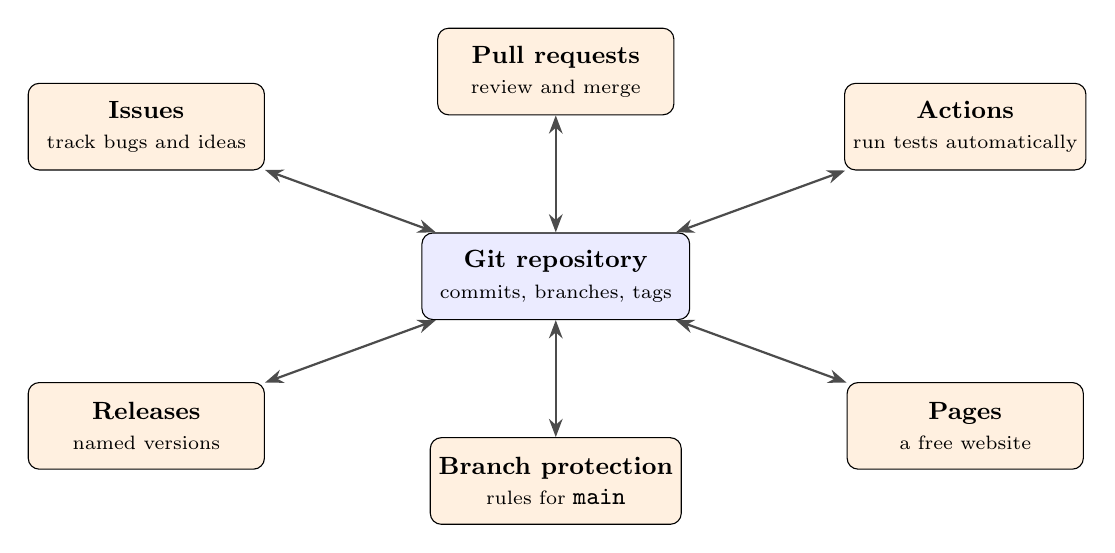
\begin{tikzpicture}
  \node[gitb] (git) at (0,0) {\textbf{Git repository}\\\scriptsize commits, branches, tags};
  \node[feat] (iss) at (-5.2,1.9) {\textbf{Issues}\\\scriptsize track bugs and ideas};
  \node[feat] (prs) at (0,2.6) {\textbf{Pull requests}\\\scriptsize review and merge};
  \node[feat] (act) at (5.2,1.9) {\textbf{Actions}\\\scriptsize run tests automatically};
  \node[feat] (rel) at (-5.2,-1.9) {\textbf{Releases}\\\scriptsize named versions};
  \node[feat] (pro) at (0,-2.6) {\textbf{Branch protection}\\\scriptsize rules for \code{main}};
  \node[feat] (pag) at (5.2,-1.9) {\textbf{Pages}\\\scriptsize a free website};
  \foreach \n in {iss,prs,act,rel,pro,pag} { \draw[link,<->] (git)--(\n); }
\end{tikzpicture}
\caption{The Git repository at the centre, GitHub's features around it. This lecture covers all of the orange boxes except pull requests (Lecture 7).}
\label{fig:features}
\end{figure}

\section{Issues: tracking what needs doing}

An \textbf{issue} is a numbered discussion about one thing: a bug, a question, an idea. Issues turn ``someone should fix this'' into a visible to-do list. Create one with \textbf{Issues $\rightarrow$ New issue}.

\begin{itemize}
  \item A good \textbf{title} says what is wrong in one line: \emph{Greeting prints ``Helo'' instead of ``Hello''}.
  \item A good \textbf{description} says how to see the problem, what you expected, and what happened.
  \item \textbf{Labels} classify (\emph{bug}, \emph{enhancement}, \emph{good first issue}); \textbf{assignees} say who works on it; \textbf{milestones} group issues for a version.
\end{itemize}

Issues and pull requests share the numbering: \code{\#12} anywhere in a comment or description becomes a link to issue or pull request number 12, and \code{@name} notifies a person. Descriptions are written in Markdown, so a task list works as a checklist:

\begin{lstlisting}
- [x] reproduce the bug
- [ ] write a fix
- [ ] add a test
\end{lstlisting}

\subsection{Closing issues automatically}

When a pull request fixes an issue, you do not have to close the issue by hand. Put a \textbf{closing keyword} followed by the issue number in the pull request's description (or in a commit message):

\begin{lstlisting}
Fix greeting typo

Closes #12
\end{lstlisting}

The keywords are \emph{close(s/d)}, \emph{fix(es/ed)} and \emph{resolve(s/d)}, in any capitalisation. The issue is closed \textbf{when the change is merged into the default branch} (usually \code{main}), not when the pull request is opened. Before that, the issue page shows the pull request as linked.

\begin{figure}[H]
\centering
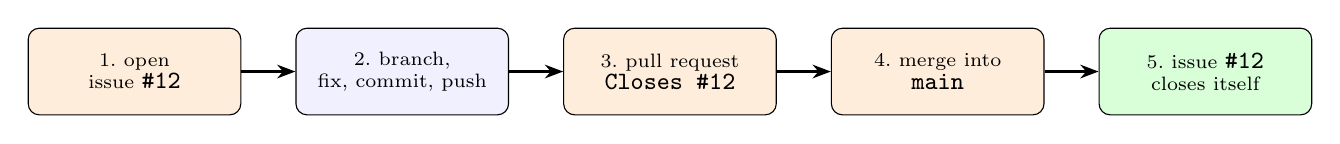
\begin{tikzpicture}[
  blk/.style={draw,rounded corners,fill=blue!6,minimum width=2.7cm,minimum height=11mm,align=center,font=\scriptsize,inner sep=3pt},
  hum/.style={blk,fill=orange!14},
  arr/.style={->,thick,>=Stealth}]
  \node[hum] (a) at (0,0) {1.\ open\\issue \code{\#12}};
  \node[blk] (b) at (3.4,0) {2.\ branch,\\fix, commit, push};
  \node[hum] (c) at (6.8,0) {3.\ pull request\\\code{Closes \#12}};
  \node[hum] (d) at (10.2,0) {4.\ merge into\\\code{main}};
  \node[hum,fill=green!15] (e) at (13.6,0) {5.\ issue \code{\#12}\\closes itself};
  \draw[arr] (a)--(b); \draw[arr] (b)--(c); \draw[arr] (c)--(d); \draw[arr] (d)--(e);
\end{tikzpicture}
\caption{Issue to fix to closed issue. Orange steps happen on the website, blue steps are the Git commands you know.}
\label{fig:issue}
\end{figure}

\subsection{Templates and the \texttt{.github} folder}

GitHub looks in a folder called \code{.github} in your repository for helper files. Two are very useful for teamwork:

\begin{itemize}
  \item \code{.github/ISSUE\_TEMPLATE/bug\_report.md}: pre-fills the form when someone opens an issue.
  \item \code{.github/pull\_request\_template.md}: pre-fills every pull request description.
\end{itemize}

A template for bug reports starts with a block of settings between lines of three dashes, called \emph{front matter}, followed by Markdown:

\begin{lstlisting}
---
name: Bug report
about: Something does not work
---

## What happened?

## What did you expect?
\end{lstlisting}

and a pull-request template is plain Markdown, for example:

\begin{lstlisting}
## What does this change?

## Checklist
- [ ] The tests pass
- [ ] I read my own diff
\end{lstlisting}

These files are ordinary files: you commit and push them like any other, and they take effect on the default branch.

\begin{quickfact}
GitHub also offers \emph{Projects}: a board with columns (to do, doing, done) whose cards are issues and pull requests. It is optional; many small teams get by with labels.
\end{quickfact}

\section{GitHub Actions: letting a robot run your tests}

\textbf{Continuous integration} (CI) means: every time someone pushes, a machine automatically builds and tests the project, and reports the result next to the commit. Nobody forgets to run the tests, and a broken change is caught before it is merged. On GitHub this is done by \textbf{Actions}.

You describe what to run in a \textbf{workflow file}: a text file in the folder \code{.github/workflows/}, written in \textbf{YAML}. YAML is a simple format of \code{key: value} pairs where \emph{indentation} (spaces, never tabs) shows nesting. Our project has a test script \code{test.sh}; this workflow runs it:

\begin{lstlisting}
name: CI
on:
  push:
    branches: [main]
  pull_request:
jobs:
  test:
    runs-on: ubuntu-latest
    steps:
      - uses: actions/checkout@v4
      - name: Run the tests
        run: bash test.sh
\end{lstlisting}

Line by line:

\begin{center}
\small
\begin{tabular}{@{}l >{\raggedright\arraybackslash}p{10.2cm}@{}}
\toprule
Line & Meaning \\
\midrule
\code{name: CI} & The name shown in the Actions tab. \\
\code{on:} & \emph{When} to run: on every push to \code{main}, and on every pull request. \\
\code{jobs:} / \code{test:} & A job called \code{test}. A workflow can have several; they run in parallel. \\
\code{runs-on: ubuntu-latest} & The kind of computer GitHub lends you: a fresh virtual machine with Linux. \\
\code{steps:} & The job's steps, run in order. A line starting with \code{-} begins a step. \\
\code{uses: actions/checkout@v4} & Use a ready-made \emph{action}: it downloads your repository into the machine. (Without it the machine has no files.) \\
\code{run: bash test.sh} & Run a command, exactly as in your terminal. If it fails (non-zero exit), the job fails. \\
\bottomrule
\end{tabular}
\end{center}

\begin{figure}[H]
\centering
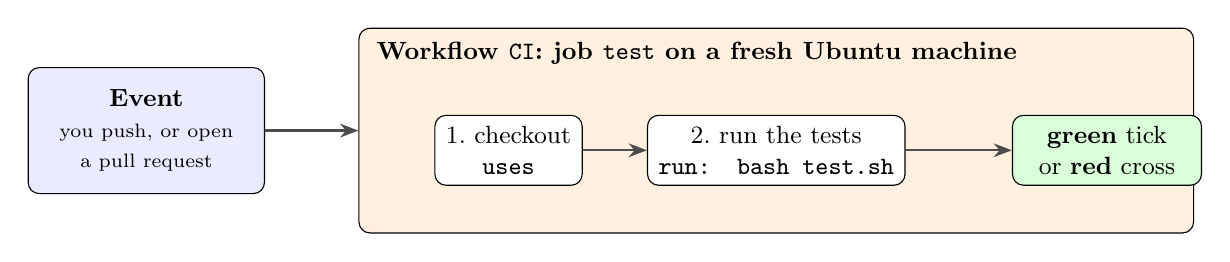
\begin{tikzpicture}[
  box/.style={draw,rounded corners,align=center,font=\small,inner sep=4pt}]
  \node[box,fill=blue!8,minimum width=3.0cm,minimum height=1.6cm] (ev) at (0,0) {\textbf{Event}\\\scriptsize you push, or open\\\scriptsize a pull request};
  \node[box,fill=orange!12,minimum width=10.6cm,minimum height=2.6cm] (wf) at (8.0,0) {};
  \node[font=\small\bfseries,anchor=north west] at (2.8,1.25) {Workflow \code{CI}: job \code{test} on a fresh Ubuntu machine};
  \node[box,fill=white] (s1) at (4.6,-0.25) {1.\ checkout\\\scriptsize \code{uses}};
  \node[box,fill=white] (s2) at (8.0,-0.25) {2.\ run the tests\\\scriptsize \code{run: bash test.sh}};
  \node[box,fill=green!15,minimum width=2.4cm] (res) at (12.2,-0.25) {\textbf{green} tick\\or \textbf{red} cross};
  \draw[link] (ev)--(wf.west); \draw[link] (s1)--(s2); \draw[link] (s2)--(res);
\end{tikzpicture}
\caption{What happens on a push: the event starts the workflow, a fresh virtual machine runs the steps, and the result appears on the commit and the pull request.}
\label{fig:actions}
\end{figure}

\textbf{Using it.} Commit the file \code{.github/workflows/ci.yml} and push. Open the \textbf{Actions} tab of your repository: the run appears, yellow while it works, then a green tick or a red cross. Click it to read the log of every step. On a pull request the same result is shown as a \emph{check} next to the merge button. If a step fails, read its log, fix the problem, and push again: the workflow runs again.

\begin{pitfall}
\textbf{YAML is picky.} Use spaces, never tabs. Keep the indentation exactly as shown: a step moved by one space changes its meaning. A broken file does not run at all; the Actions tab then shows an error with the line number.
\end{pitfall}

\begin{quickfact}
Actions are free for public repositories; private repositories get a limited monthly allowance of free minutes. The version after \code{@} (\code{v4}) pins the action's major version; newer major versions appear over time, and GitHub's documentation lists the current one. Never write passwords into a workflow file; secrets go under Settings $\rightarrow$ Secrets and variables $\rightarrow$ Actions and are used as \code{\$\{\{ secrets.NAME \}\}}.
\end{quickfact}

\section{Branch protection: guarding \texttt{main}}

In Lecture 8 you learned that rewriting a shared branch is dangerous, and in Lecture 7 that changes should be reviewed. \textbf{Branch protection} makes GitHub enforce this. In the repository's \textbf{Settings} (under \emph{Branches}, or \emph{Rules}) you can add a rule for \code{main}. The most useful options:

\begin{center}
\small
\begin{tabular}{@{}l >{\raggedright\arraybackslash}p{9.4cm}@{}}
\toprule
Option & Effect \\
\midrule
Require a pull request before merging & Nobody can push straight to \code{main}; changes arrive through reviewed pull requests. \\
Require approvals & A pull request needs at least $n$ approvals before the merge button works. \\
Require status checks to pass & The CI workflow must be green. A red cross blocks the merge. \\
Block force pushes & \code{git push --force} (even with a lease) is refused on \code{main}. \\
Restrict deletions & The branch cannot be deleted. \\
\bottomrule
\end{tabular}
\end{center}

Together they give the team's central rule: \emph{nothing reaches \code{main} unless it was reviewed and the tests pass}. (Branch protection is available for public repositories on every plan; for private repositories it depends on your plan.)

\section{Tags and releases: naming a version}

A branch label moves every time you commit. Sometimes you need a label that \emph{stays put}: ``this exact commit is version 1.0.0''. That is a \textbf{tag}.

\begin{figure}[H]
\centering
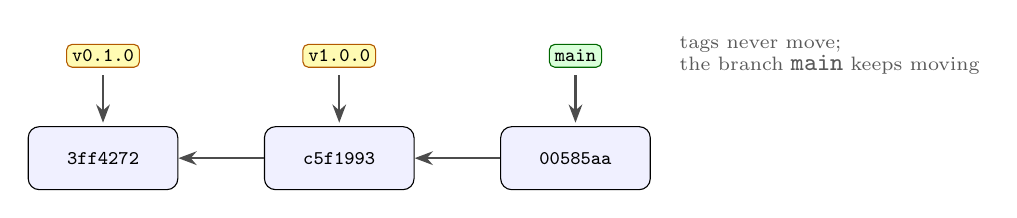
\begin{tikzpicture}
  \node[cbx] (a) at (0,0) {3ff4272}; \node[cbx] (b) at (3.0,0) {c5f1993}; \node[cbx] (c) at (6.0,0) {00585aa};
  \draw[link] (b)--(a); \draw[link] (c)--(b);
  \node[tag,fill=yellow!30,draw=orange!70!black] at (0,1.3) {v0.1.0}; \draw[link] (0,1.05)--(0,0.45);
  \node[tag,fill=yellow!30,draw=orange!70!black] at (3.0,1.3) {v1.0.0}; \draw[link] (3.0,1.05)--(3.0,0.45);
  \node[branchtag] at (6.0,1.3) {main}; \draw[link] (6.0,1.05)--(6.0,0.45);
  \node[font=\scriptsize,anchor=west,text=black!65,align=left] at (7.2,1.3) {tags never move;\\the branch \code{main} keeps moving};
\end{tikzpicture}
\caption{Tags mark specific commits. After more commits, \code{main} has moved on, but \code{v1.0.0} still names the same commit.}
\label{fig:tags}
\end{figure}

There are two kinds. A \textbf{lightweight} tag is just a name for a commit. An \textbf{annotated} tag is a small object of its own that also stores who made it, when, and a message; use annotated tags for releases.

\begin{lstlisting}
$ git tag v0.1.0 3ff4272              # lightweight, on a given commit
$ git tag -a v1.0.0 -m "First release"    # annotated, on the current commit
$ git tag -n                          # list tags with their messages
v0.1.0          Add README
v1.0.0          First release
$ git show v1.0.0
tag v1.0.0
Tagger: Practice User <practice@example.com>

First release

commit <40-character ID>
...
\end{lstlisting}

\textbf{Tags are not pushed automatically.} Send them explicitly:

\begin{lstlisting}
$ git push origin v0.1.0 v1.0.0        # or: git push origin --tags   (all tags)
 * [new tag]         v0.1.0 -> v0.1.0
 * [new tag]         v1.0.0 -> v1.0.0
\end{lstlisting}

Other tag commands: \code{git tag -d v1.0.0} deletes a local tag, \code{git push origin --delete v1.0.0} deletes it on the remote, and \code{git describe} tells you how far the current commit is from the nearest tag:

\begin{lstlisting}
$ git describe --tags
v1.0.0-1-g00585aa           # one commit after v1.0.0
$ git switch --detach v0.1.0
HEAD is now at 3ff4272 Add README
\end{lstlisting}

Checking out a tag puts you on a detached \code{HEAD}, exactly as in Lecture 4: good for looking at the old version, not for committing.

\subsection{Version numbers}

Most projects use \textbf{semantic versioning}: \code{MAJOR.MINOR.PATCH}.

\begin{center}
\small
\begin{tabular}{@{}l l l@{}}
\toprule
You made & Bump & From \code{1.0.0} to \\
\midrule
a bug fix, nothing else changes & PATCH & \code{1.0.1} \\
a new feature that does not break anything & MINOR & \code{1.1.0} \\
a change that breaks how people use it & MAJOR & \code{2.0.0} \\
\bottomrule
\end{tabular}
\end{center}

A \textbf{release} is GitHub's page for a tag. Under \textbf{Releases $\rightarrow$ Draft a new release} you choose a tag, write a title and notes (the button \emph{Generate release notes} lists the merged pull requests for you), optionally attach files, and press \emph{Publish release}. GitHub automatically adds downloadable ZIP and tar archives of the source code at that tag.

\section{GitHub Pages and a healthy repository}

\textbf{GitHub Pages} publishes files from your repository as a website, for free. In \textbf{Settings $\rightarrow$ Pages} choose to deploy from a branch (for example \code{main}, folder \code{/} or \code{/docs}). After a minute the site is at \code{https://YOURNAME.github.io/REPOSITORY/}. A single \code{index.html} (or \code{index.md}) is enough. It is a good place for project documentation or a personal page.

A repository that others can use usually contains:

\begin{itemize}
  \item \code{README.md}: what it is and how to use it (shown on the front page);
  \item \code{LICENSE}: what others may do with the code (GitHub's \emph{Add file} menu offers common licences; without one, the default is ``all rights reserved'');
  \item \code{.gitignore} (Lecture 2) and, for teamwork, \code{CONTRIBUTING.md} (how to propose changes) and the \code{.github} templates from above.
\end{itemize}

\begin{pitfall}
\textbf{Security basics.} Turn on two-factor authentication (Lecture 6). Never commit passwords, keys or tokens (Lecture 2): GitHub scans for known secrets, but history keeps them. GitHub's \emph{Dependabot} can warn you about vulnerable libraries in a project; enable it under Settings $\rightarrow$ Code security when you have dependencies.
\end{pitfall}

\Needspace{12\baselineskip}
\section{Homework 9}

\begin{homework}{9: Issues, CI, and a release}
\textbf{Part A: practise with a ``server'' folder} (no internet needed). The setup script creates \code{practice/hw9\_server.git}, a repository that plays the role of GitHub, holding a tiny project whose test fails because of a typo. From the course folder:
\begin{lstlisting}
$ bash codeHints/L09/setup_hw9.sh
$ cd practice
\end{lstlisting}
Do the tasks in order. To start over: \code{setup\_hw9.sh --reset} from the course folder.

\begin{description}[leftmargin=1.2em,style=nextline]
\item[9.1 Clone] Clone the server into \code{hw9} and go in. Set your name and email (\code{git config user.name} ...) if they are not set globally.
\item[9.2 See the failure] Run \code{bash test.sh}. It prints \code{FAIL}: this is what CI would show as a red cross.
\item[9.3 Fix it] Correct the typo in \code{greet.sh} so that \code{bash test.sh} prints \code{PASS}.
\item[9.4 Closing keyword] Commit the fix with a message that has the subject \code{Fix greeting typo} and a second paragraph \code{Closes \#1}: \code{git commit -m "Fix greeting typo" -m "Closes \#1"}.
\item[9.5 The workflow] Create \code{.github/workflows/ci.yml} (use the example of this lecture: it checks out the code and runs \code{bash test.sh}, on pushes to \code{main} and on pull requests). Spaces only, no tabs. Commit it as \code{Add CI workflow}.
\item[9.6 Templates] Create \code{.github/ISSUE\_TEMPLATE/bug\_report.md} (front matter with \code{name:} and \code{about:}, then at least one \code{\#\#} heading) and \code{.github/pull\_request\_template.md} (with a checklist line \code{- [ ] ...}). Commit them as \code{Add templates}.
\item[9.7 Tags] Create the \emph{lightweight} tag \code{v0.1.0} on the very first commit (\code{git rev-list --max-parents=0 HEAD} prints its ID) and the \emph{annotated} tag \code{v1.0.0} (message \code{First release}) on your newest commit. Push everything: \code{git push origin main v0.1.0 v1.0.0}.
\item[9.8 Questions] In \code{practice/hw9\_answers.txt} (next to \code{hw9}; create it with \code{printf} or \code{echo}) write \code{next-bugfix=<version>} (the next version number after fixing another bug in \code{1.0.0}) and \code{issue-closes-when=<opened or merged>} (when does \code{Closes \#12} close issue 12?).
\end{description}

\textbf{Part B: the real thing on GitHub} (optional, but this is the point). You need your GitHub account and SSH key (Lecture 6).
\begin{description}[leftmargin=1.2em,style=nextline]
\item[9.9 Publish and watch CI] On GitHub create a new \emph{Public} repository \code{ci-practice} \emph{without} a README. In \code{practice/hw9} run \code{git remote add github <your address>} and \code{git push github main v0.1.0 v1.0.0}. Open the \textbf{Actions} tab: your workflow ran. Add the line \code{repo=<you>/ci-practice} to \code{hw9\_answers.txt}.
\item[9.10 Issue to pull request to closed issue] \emph{Now} (after the push) create Issue \#1 (use the bug template; title: \emph{Add a note to the README}). In \code{hw9} create a branch \code{readme-note}, add a line to \code{README.md}, commit, and \code{git push github readme-note}. Open a pull request into \code{main} with the description \code{Closes \#1}; wait for the green check; merge it. Issue \#1 should close by itself. Add \code{issue=1} to the answers file. (Create the issue only \emph{after} the first push: the old commit \code{Closes \#1} would otherwise close it at once.)
\item[9.11 Release] On GitHub open \textbf{Releases $\rightarrow$ Draft a new release}, choose the tag \code{v1.0.0}, press \emph{Generate release notes}, and publish.
\item[9.12 Explore (not checked)] Under Settings, look at branch protection and GitHub Pages. In Settings you can also protect \code{main} so that CI must pass.
\end{description}

\textbf{Check yourself:} from the course folder run \code{bash codeHints/L09/check\_hw9.sh}. Part A needs no network. Part B is checked if \code{hw9\_answers.txt} contains \code{repo=}; the checker reads your public repository through GitHub's public interface (your issue, release and latest Actions run) and says so if it cannot reach GitHub. Then compare with the solutions at the end of this lecture.
\end{homework}

\section{Summary}

\begin{itemize}
  \item Issues track work; \code{Closes \#12} in a pull request closes the issue when the change reaches \code{main}. Templates live in \code{.github/}.
  \item Actions run a YAML workflow from \code{.github/workflows/} on each push or pull request: \code{on}, \code{jobs}, \code{runs-on}, \code{steps}, \code{uses}, \code{run}. Green tick or red cross.
  \item Branch protection (pull request, approvals, passing checks, no force push) enforces the team's rules on \code{main}.
  \item Tags name fixed commits (annotated for releases; push them explicitly); releases are GitHub pages for tags; version as \code{MAJOR.MINOR.PATCH}. Pages publishes a free website. (Further reading: GitHub Docs, ``About issues'', ``Understanding GitHub Actions''; \emph{Pro Git}, Chapter 2.6.)
\end{itemize}


\solutionspage

\section*{Solutions to Homework 9}

\textbf{Part A.}

\begin{lstlisting}
$ bash codeHints/L09/setup_hw9.sh
$ cd practice
$ git clone hw9_server.git hw9
$ cd hw9
$ bash test.sh
FAIL: got 'Helo, world'
$ sed -i.bak 's/Helo/Hello/' greet.sh && rm greet.sh.bak    # or edit by hand
$ bash test.sh
PASS
$ git commit -am "Fix greeting typo" -m "Closes #1"
$ mkdir -p .github/workflows .github/ISSUE_TEMPLATE
\end{lstlisting}

Create \code{.github/workflows/ci.yml} (spaces only):

\begin{lstlisting}
name: CI
on:
  push:
    branches: [main]
  pull_request:
jobs:
  test:
    runs-on: ubuntu-latest
    steps:
      - uses: actions/checkout@v4
      - name: Run the tests
        run: bash test.sh
\end{lstlisting}

Create \code{.github/ISSUE\_TEMPLATE/bug\_report.md} (the front matter with \code{name:} and \code{about:} and the two headings of the lecture) and \code{.github/pull\_request\_template.md} (the heading and the checklist of the lecture). Then:

\begin{lstlisting}
$ git add .github
$ git commit -m "Add CI workflow and templates"
$ git tag v0.1.0 $(git rev-list --max-parents=0 HEAD)
$ git tag -a v1.0.0 -m "First release"
$ git push origin main v0.1.0 v1.0.0
$ printf 'next-bugfix=1.0.1\nissue-closes-when=merged\n' > ../hw9_answers.txt
\end{lstlisting}

(Committing the workflow and the templates in two commits, as the task text says, works equally well.)

\textbf{9.3--9.4.} The checker runs your project's \code{test.sh} on a copy of the server's \code{main}, which is exactly what the workflow does on GitHub. \code{git commit -m ... -m ...} makes the second \code{-m} a separate paragraph of the message; GitHub looks for the keyword and the issue number anywhere in it.

\textbf{9.5.} Without \code{uses: actions/checkout} the virtual machine would have no files, so \code{bash test.sh} would fail. The workflow file must be in \code{.github/workflows} (with an \emph{s}).

\textbf{9.7.} The lightweight tag is a bare name for the first commit; the annotated tag has its own object with your message, so \code{git show v1.0.0} shows a \emph{Tagger}. Tags are only pushed when you name them (or use \code{--tags}).

\textbf{9.8.} Fixing a bug in \code{1.0.0} gives the patch version \code{1.0.1}. \code{Closes \#12} closes the issue when the change is \emph{merged} into the default branch, not when the pull request is opened.

\textbf{Part B.}

\begin{lstlisting}
(GitHub) New repository: ci-practice, Public, no README
$ git remote add github git@github.com:YOURNAME/ci-practice.git
$ git push github main v0.1.0 v1.0.0
(GitHub) Actions tab: the "CI" workflow ran: green tick
$ printf 'repo=YOURNAME/ci-practice\n' >> ../hw9_answers.txt
(GitHub) Issues > New issue "Add a note to the README"  -> number 1
$ git switch -c readme-note
$ echo "Notes coming soon." >> README.md
$ git commit -am "Add a note to the README"
$ git push github readme-note
(GitHub) Open the pull request, description "Closes #1"; wait for the green check; Merge
(GitHub) Issue #1 is now closed
$ printf 'issue=1\n' >> ../hw9_answers.txt
(GitHub) Releases > Draft a new release > tag v1.0.0 > Generate release notes > Publish
\end{lstlisting}

Replace \code{YOURNAME} with your GitHub user name. The checker needs the answers file to contain \code{repo=}, \code{issue=}, and a remote of \code{practice/hw9} that points at that repository. It then asks GitHub's public interface whether the issue is closed, whether a release exists for \code{v1.0.0}, and whether the latest Actions run on \code{main} succeeded. If the last check is red, open the run's log in the Actions tab.

\Needspace{8\baselineskip}
\textbf{Common mistakes.}
\begin{itemize}
  \item A \emph{tab} character in the workflow (the checker reports it) or a folder called \code{.github/workflow} instead of \code{workflows}.
  \item Creating Issue \#1 \emph{before} the first push: the old commit message \code{Closes \#1} then closes it at once, and the pull request closes nothing. The check passes anyway, but you missed the exercise. Push first, then create the issue.
  \item Forgetting to push the tags: \code{git push origin main} sends no tags.
  \item Creating the GitHub repository with a README: the first push is rejected because the histories differ. Create it empty.
  \item A private repository: GitHub's public interface cannot see it, so the checker reports that it cannot find it.
  \item Writing \code{issue-closes-when=opened}: the issue closes when the change is \emph{merged}.
\end{itemize}


\end{document}
